\newthought{Neuroscience as a whole} is concerned with the function of the nervous system. More precisely, it asks a very simple question: {\em What is the brain 
doing?}\footnote{ Or alternatively: {\em What is the nervous system doing?}} The simplicity with which humans and animals perform in their environment makes it 
almost unnatural to ask how their brains enable these behaviors. It is often hard to explain to laymen the complexity involved in preparing even the simplest actions, 
such as saccades or walking, such is the ease with which these are normally performed. Although one can not realistically expect to answer that question in any 
general fashion, I will try to touch upon a number of points which shed light on some aspects of the nervous system and provide us with a {\em guiding principle} to 
understand what the brain is doing, why and possibly how.\par

Neuroscience was born as a branch of biology, and although it is now often thought of as  an interdisciplinary science in itself, its objects of study are still to the 
largest extent biological systems. Theodosius Dobzhansky published an influential essay in 1973, entitled {\em Nothing in biology makes sense except in the light of 
evolution},\cite{Dobzhansky1973} which defends exactly that point. Though it has been reviewed and revisited constantly since its proposal, the theory of evolution 
through natural selection remains the central pillar of biological sciences. As such, neuroscience must also view its objects of study through the lenses of evolution. 
More specifically, we can then ask ourselves {\em What evolutionary advantage would this brain bring to an individual?} instead of {\em Why is the brain this way?} 
That being said,  there are caveats in the case of neuroscience. For one, the brain is capable of plasticity and adaptation unthinkable for other organs, and so we can 
not expect to understand the functionality of the brain in the same way in which the shape of bird beaks can be understood as a function of their preferred fruits and 
seeds. Furthermore, the brain controls all of the motor and perceptual apparatus, having a multitude of uses and purposes, unlike simpler organs.\par

One particular aspect of the brain which has received increasing attention recently is its ability to deal with uncertainty. In a very fruitful line of research, a number 
of experiments have demonstrated that humans and animals integrate uncertain information in a near-optimal way. The so-called {\em Bayesian Brain},\cite{Knill2004} 
would explicitly represent the distribution over world states and perform inference in a manner consistent with Bayesian inference, obtaining optimal integration of 
sensory cues from different modalities, for example. It is still a matter of debate how these Bayesian computations would be implemented in the brain. One possibility 
is that the activity of neurons is sampling from a representation of the distribution of world states,\cite{Berkes2011} which is frequently called the {\em sampling 
hypothesis}. Another is that the activity of the neurons itself represents the likelihood over world states,\cite{Ma2006} and the population as a whole codes for the 
distribution, hence the term {\em population coding}.\par

\subsection*{Structure}

\newthought{The main goal of this thesis} is to develop a conceptual framework for studying optimal population coding in a dynamic framework. Furthermore, I will
establish a link between optimal dynamic encoders and the efficient coding hypothesis, first proposed by Horace Barlow.\cite{Barlow1961} I believe that the 
inclusion of time into the coding framework raises a number of questions, which have not been addressed in the scientific literature properly. In the remainder of this 
chapter, I will discuss the efficient coding hypothesis and its more recent developments, and I will touch upon its relationship to Shannon's information theory.\cite{Shannon1948} I will finish by discussing the issue of dynamic population coding, highlighting the issues which I believe are of importance in considering the 
temporal aspect of coding. I will make the case for a study of optimal filtering of partially observed stimuli as a model of stimulus inference based on spike trains. 
Following, in \fref{chap:filtering}  I will introduce the general theory of filtering of stochastic stimuli. After that, in \fref{chap:MSE} I will discuss results regarding the 
Mean-Squared-Error (MSE) of optimal filters of point process data, presenting a number of new analytical results. In \fref{chap:control}, I will generalize the filtering 
framework to control problems, showing results for optimal control theory of point process-observed processes. In \fref{chap:optimal} I will then provide the connection 
to neuroscience, by considering the optimal encoding strategy for a population of neurons coding for a stochastic stimulus. I will then finalize by discussing the impact 
of the work presented and suggesting future research directions.\par

\subsection*{Contribution}

\newthought{The main contribution of this thesis} is in providing a conceptual toolbox to study optimal coding problems in a dynamic environment. I propose that the 
study of the average performance of an optimal Bayesian filter reconstructing the relevant stimulus provides a good measure of the quality of a dynamic code. Using 
this framework, I derive analytical results for the fast population code for dense populations of Gaussian neurons proposed by Quentin Huys.\cite{Huys2007} These are 
to my best knowledge the first results of this kind obtained for temporal coding of dynamic stimuli.\par

The results presented in this thesis have been published and presented throughout the duration of my doctoral studies. The findings in \fref{chap:MSE} were first
published at the \emph{Neural Information Processing Systems} conference, where it was presented as a poster in addition to the publication in the conference 
proceedings \citep{Susemihl2011a}. These results were then further developed and put in the greater context of computational neuroscience and published in a special
edition of the \emph{Journal of Statistical Mechanics: Theory and Experiment} title \emph{Statistical Physics and Neuroscience}, focusing on the challenges 
neuroscience presented to statistical physics \citep{Susemihl2012a}. The results presented \fref{chap:control} have been submitted to the \emph{NIPS} conference
proceedings as well, and are currently under review.\par

Parallelly to the topics presented here I have also contributed to other ongoing research projects during my doctoral studies. In a research project headed by 
fellow doctoral student Chris H\"ausler and myself, we have proposed a novel way of training temporal Boltzmann machines, which improves their performance as
generative models of temporal data greatly. This was presented in a workshop on Deep Learning at the \emph{NIPS} conference as well \citep{hausler2012b}. This was
then used as a model for temporal sparsity in visual cortex and results on sequences of natural images were published in the journal \emph{Brain Research} in a
special issue on neural coding \citep{Hausler2013a}. The advantages of the training procedure for generative models of temporal data as well as for forecasting were
further extended on and submitted for publication in the journal \emph{Neurocomputing} \citep{Hausler2013b}.\par

In addition to these projects, I have also worked on the publication of a manuscript originating from my Masters thesis, which was since published in the journal 
\emph{Physica A}. There we investigated the effect of different learning strategies on the emergence of moral opinions in a model of social learning  
\citep{Vicente2014}.

\section{Efficient Coding Hypothesis}

\newthought{In information theory, the information} associated with a random event is defined as the logarithm of its inverse probability. We can further define the 
entropy of a distribution 
over a set of events as the average information conveyed by these events. So if we have a random variable $X$ taking values $x \in \mathcal{A}_X$ and a probability 
distribution $P_X : \mathcal{A}_X \to [0,1]$, we will have\footnote{Abusing the notation to allow for $0\log(0) = 0$.}
$$
H(X)= \sum_x P_X(x) \log\left(\frac{1}{P_X(x)}\right) = - \sum_x P_X(x) \log\left({P_X(x)}\right).
$$
The entropy measures how much information is gained from a random observation of $X$ on average, and is usually thought of as a measure of the uncertainty or 
disorder in the distribution $P_X$. Its unit is usually defined as the {\em bit} when the logarithm is taken in base 2, contracted from \emph{binary digit}. So, a distribution where 
we have $P_X(x^*) = 1$ for some $x^*$ and $P_X(x) = 0$ for all other $x\neq x^*$ would have an entropy of $0$, since our measurement gives us an average 
information of $0$. The outcome $x^*$ is completely non-informative, and all other outcomes, while infinitely informative have a zero probability of happening.\par
It can also easily be seen that in the absence of other constraints, if the set of outcomes $\mathcal{A}_X$ is finite, the entropy is maximized by the uniform 
distribution over outcomes $x$, which would give us the maximal average information per observation of the variable $X$.\footnote{We provide a short demonstration in 
\fref{app:entropy}} In information theory, the entropy provides the number of bits it takes, on average, to specify an outcome of the random variable $X$.\par
We can now define the conditional entropy of two random variables $X$ and $Y$ as
$$
H(Y|X) = \sum_x P_X(x) \sum_y P_Y(y|x) \log\left(\frac{1}{P_Y(y|x)}\right),
$$
i.e. the conditional entropy is the average entropy of $Y$ given $X$, averaged over $X$. This gives us the remaining uncertainty in $Y$ after $X$ has been observed averaged over all outcomes of $X$, or alternatively, the number of bits required to code for an outcome of $Y$ given an outcome of $X$, on average. Let us also define the mutual information between $Y$ and $X$ as
$$
I(X;Y) = H(Y) - H(Y|X) = H(X) - H(X|Y) = I(Y;X).
$$
In line with our interpretation of the conditional entropy, this would give us the average reduction of uncertainty in $Y$ given the observation of $X$ or vice-versa. Note that, if we fix the distribution of $X$ (or $Y$), the mutual information is always maximized if the conditional entropy $H(X|Y)$ (or $H(Y|X)$, respectively) is minimized. It is easy to see that if $P_X(x|y)$ ($P_Y(y|x)$) is given by a one-to-one mapping between $X$ and $Y$, the conditional entropy is zero, as no uncertainty is left in $X$ after the observation of $Y$ (no uncertainty in $Y$ is left after the observation of $X$).\par
Shannon regarded a noisy communication channel as a set of two random variables, one representing the codeword to be transmitted ($X$) and another representing the message received ($Y$). The noise in the channel would then be given by the conditional distribution of received messages given the transmitted codewords ($P_Y(y|x)$). The capacity of this channel is then given by
$$
C = \max_{P_X} I(X;Y).
$$
This is the maximum amount of information we can transmit through a noisy channel given by the distribution $P_Y(Y|X)$.
The rate of a given code is given by the number of bits needed to represent $X$ divided by the number of bits needed to represent $Y$, so if to send a one-bit message $x$ we must transmit a three-bit codeword $y$, our code would have a rate of $1/3$.
The noisy-channel coding theorem\cite{mackay2003information} then states
\newtheorem{noisychannel}{Theorem}
\begin{noisychannel}
\label{thm:noisychannel}
For every discrete memoryless channel with capacity $C$, for any $\epsilon>0$, any rate $R<C$, and for large enough $N$, there exists a code of length $N$ and rate $\leq R$ and a decoding algorithm such that the maximal probability of %block 
error is $\epsilon$.
\end{noisychannel}
Before Shannon's work, it was generally believed that to achieve a vanishingly small error one would need a code with vanishingly small rate. The theorem shows, however, that one can achieve any rate below the channel capacity asymptotically.\par
Shannon's work had profound impacts throughout science and technology. In the field of neuroscience, Fred Attneave was probably the first to propose the use
of information-theoretical concepts in the study of vision.\cite{Attneave1954} His was a very informal approach though, mostly dedicated at showing how humans
compress visual information in a way consistent with Shannon's ideas. Horace Barlow proposed an information-theoretical approach to the function of sensory
relays. He consider three hypotheses, discarding the first two and concluding that one function of sensory relays must be to reduce the redundancy of the
representation of sensory input. Furthermore, he introduced a notion of metabolic efficiency into Shannon's ideas, noting that instead of allocating fewer bits to
frequent codewords as in general coding theory, a neural system would allocate fewer \emph{spikes} to frequent stimuli. The redundancy of a code is given by
$$
\mathcal{R} = 1 - \frac{I(X;Y)}{C},
$$
and it quantifies how {\em efficiently} a given code encodes codewords $x$ into messages $y$. Note that in the case of a noiseless channel, this reduces to 
$$
\mathcal{R} = 1 - \frac{H(X)}{C}= 1 - \frac{H(Y)}{C} = 0.
$$
The {\em efficient coding hypothesis}, first proposed by Barlow\cite{Barlow1961} states that sensory relays in the nervous system recode the	messages to reduce the redundancy in them. This allows us to relate the distribution of the codewords in nature, given by the stimulus statistics, to the firing statistics of the nervous system.\par
In one popular example, Simon Laughlin related the distribution of contrasts in the natural environment of the blowfly to the tuning function of the large monopolar 
cells (LMC's) in the blowfly's visual system.\cite{Laughlin1981} These cells respond to the contrast level in a specific area of the visual field with a graded change
in their membrane potential, as opposed to spiking cells. Depending on the contrast of the visual stimulus they either hyperpolarize or depolarise (see the inlay in
\fref{fig:laughlin}. The nature of these responses sets a limit on the range of responses available to the neuron, namely the reversal potential of its membrane
channels, which lead to hyper- and depolarisation.
Since we are considering only one neuron, the analysis is somewhat simplified. Let us also assume that the activity of the neuron $o$ can be restricted between no response and a maximal response $o_{max}$. We can then write the activity of the neuron as a function of the contrast $c$ as $o = g(c)$. We will then have that the redundancy of the firing is given by
$$
\mathcal{R} = \frac{1}{C} \left(C - H(O) \right),
$$
which is maximized when all output levels are equally probable.
The transformation from contrasts to firing rates can be written as a simple change of variables and we have, after setting $P(o) = \alpha$\marginnote{This is a reverse application of the inverse transform method.}
$$
P(o) do = P(c) dc, \textrm{ and therefore } o(c) = \frac{1}{\alpha} \int_{-1}^c P(c') dc',
$$
as is shown in \fref{fig:laughlin}. This can be generalized to a number of cases, and Atick\cite{Atick1992} provided a thorough review of the framework.\par

\begin{marginfigure}
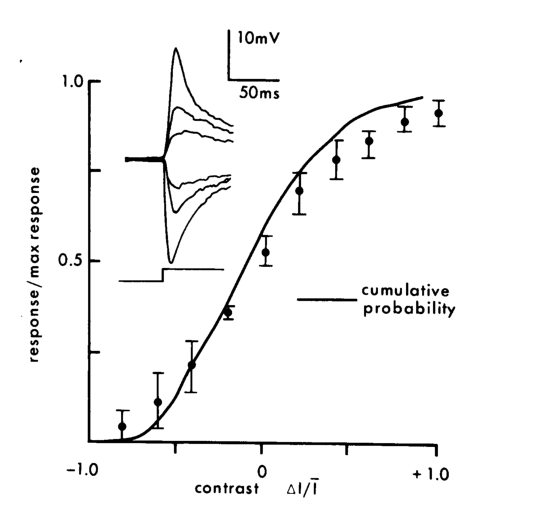
\includegraphics[width=\columnwidth]{figures/laughlin_81.eps}
\label{fig:laughlin}
\caption{The response function of the blowfly LMC closely resembles the cumulative distribution of visual contrasts in its natural environment. Figure taken from Laughlin, S. (1981)}
\end{marginfigure}

This framework can also be generalized to a population of neurons. Writing $O_i$ for the random variable associated with the output activity of each neuron and $O$ for the population activity, we can decompose the redundancy into two terms, yielding
$$
\mathcal{R} = \frac{1}{C} \left(C - \sum_i H(O_i) \right) + \frac{1}{C}\left(\sum_i H(O_i) -H(O)\right).
$$
The first term accounts for redundancy arising from unequal frequency of use of different symbols and the second accounts for redundancy arising from 
correlations between the activities $O_i$. In the example above we have only had to deal with the left term, since we had only one activity and therefore no 
correlations between them. A lot of the efficient coding literature, however, has dealt with the second term, and a number of different approaches have looked 
towards independent components of natural stimuli, assuming that whitening or gain control could account for the maximization of the first term.\par

Michael Lewicki, for example, demonstrated that using independent component analysis\footnote{Indepedent Component Analysis, or ICA for short, tries to 
decompose a signal into a set of features which are statistically independent between them. This can be done by minimization of a number of different cost 
functions.} on a set of natural sounds, comprised of human speech, animal vocalizations and natural background sounds, one recovers receptive fields similar to 
the receptive fields of early auditory neurons.\cite{Lewicki2002} There have been a number of similar studies based on different efficiency measures. 
Another way to interpret Barlow's approach is to eschew information theory and to take the hypothesis that the response of sensory systems seek to represent
in a way that allows for optimal reconstruction while minimising the number of spikes employed. This approach is often called \emph{sparse coding} since the
resulting codes will show response with sparse activity in the neural population. Bruno Olshausen and David Field,\cite{Olshausen1996} for example, have shown 
that, applying the sparse coding approach to a set of natural images results in filters similar to receptive fields in primary visual cortex.\footnote{Sparsity is in 
principle given by the number of active neurons, or if the response is graded by the sum of the activities of the neurons. This leads to cumbersome mathematics
and the kurtosis of the activity is usually employed as a surrogate for the sparsity.}\par

These results and a number of other similar studies have lent considerable traction to the idea that the nervous system is adapted to encode the stimuli present in 
the animal's natural environment. This approach, however, is not without its issues. For one, the limit of Shannon's theorem, in which the redundancy of the code is 
very small, turns the code ever harder to decode. Another important point is that, although minimizing dependence between filters yields good estimates of 
receptive fields observed in the brain, neurons' activities in the brain are far from independent.\footnote{Insert citation about correlations in brain} Though the 
redundancy reduction approach has provided numerous insights as mentioned above, other ideas have emerged since.
\par

\section{The Bayesian Brain}

The finding that humans perform near-optimally\marginnote{Optimality is used in the Bayesian sense, where we mean the subjects integrate uncertain information according to Bayes' rule} when integrating uncertain cues from different senses have led neuroscientists to theorize that the brain explicitly represents distributions over world states.\cite{Ernst2002,Ma2006} In these so-called probabilistic population codes, a spike would contribute to the computation of a posterior probability over world states with a likelihood depending on its conditional probability of firing given the stimulus. This leads to a Bayesian interpretation of the activity of the brain, where the reliability of different sensory cues can be taken in account when integrating them. It can also be argued that representing the uncertainty of events in the world has an important role in decision-making, and will therefore serve as an evolutionary advantage. To use a popular example,\footnote{This example is discussed in \citep{Ma2006}.} let us consider the case of a person deciding wether or not to jump over a stream filled with piranhas. The stream is 1.8 meters wide, and the person jumps an average distance of 2.1 meters. One will be inclined to suggest jumping.\marginnote{Should you jump over a stream filled with piranhas?} Yet both the width of the stream ($w$) as the jumping distance ($j$) are estimated based on uncertain information, and therefore could be imprecise estimates (in the case of the width) or subject to random variation (in the case of the jump distance). Suppose our best guess of the width of the stream is a normal distribution with mean 1.8 meters with a standard deviation of 0.1 meters. Furthermore suppose the standard deviation of the jump distance is 0.4 meters. That would give us a probability of approximately 0.23 of falling down the cliff. So one would definitely be less inclined to jump over the stream, or would at least take preventive actions to minimize the uncertainty in both your estimate of the width of the stream and your jump.\par
From a neural perspective, we could then infer the stimulus distribution (distribution over stream widths) given the response of a neuron population and a model of its response variability. If we assume a given neuron responds according to a certain distribution $P(r|s)$\marginnote{Here we term $r$ the response and $s$ the stimulus}, the Bayesian posterior is given simply by
\[
P(s|r) = \frac{P(r|s) P(s)}{P(r)} \propto P(r|s) P(s).
\]
Assuming independent firing for a number of neurons, whose response distributions are given by $P(r_i|s)$ we would have simply
\[
P(s|\{r_1,\ldots,r_n\}) \propto P(s) \prod_i P(r_i|s).
\]
One then still has to determine the nature of the neural variability given by $P(r|s)$. This distribution is often taken to be Poisson. This means that for very short time intervals, of duration $dt$, the probability of neuron $i$ spiking would be given by a rate function $f_i(s)$, as
\[
P_{dt}(r_i|s) \approx f_i(s) dt.
\]
The true Poisson distribution for spike counts assuming the stimulus does not change during a time interval of duration $T$ is given by\marginnote{Poisson distribution}
\[
P_T(r_i|s) = \frac{e^{-f_i(s) T}f_i(s)^{r_i}}{r_i!}
\]
The rate function $f_i(s)$ is often called the tuning function of the neuron. Given a number of neurons in primary visual cortex responding to the edges of the stream, one could then estimate the stream from those responses according to a simple model as
\[
P(width|{r_1,\ldots}) \propto P(width) \prod_i P(r_i|width),
\]
and likewise obtain the mean and standard deviation of our estimate. More simply we can look for the maximum a posteriori estimator, the value of $s$ that maximises
the probability $P(width|{r_1,\ldots})$. It is often more convenient to maximise the log-probability $\log P(width|{r_1,\ldots})$. Often an additional assumption of a flat
prior is made, yielding the Maximum likelihood estimator.
\par
Note that given a distribution over visual stimuli or a distribution over stream widths, one could seek a set of tuning functions $f_i(s)$ such that the standard deviation 
of our estimate is minimal. This is clearly a very broad formulation of the problem, but it will be the central question studied in this thesis. Alternatively, one could look
directly at the (expected) cost associated with a decision (to jump or not to jump) and choose the set of functions $f_i(s)$ which minimises the future expected cost.
We will investigate the difference between these approaches as well.
\par

Why would an organism be interested in estimating the distribution of world states conditioned on the activity of its sensory systems, though? For one, there is
the finding that the best estimator for the world's state is the mean of the posterior distribution (see \fref{chap:mse}). This means that regardless of the particulars
of the response properties of the sensory system, the posterior mean gives us the world's estimate with the lowest expected quadratic error. A second important
reason is multisensorial cue integration. Let us assume we have a visual and an auditory cue for the width of said stream.\footnote{A foggy view of the opposite 
margin ($v$) and a faint voice talking from the opposite margin ($a$).} Both lead us to different estimates of the stream's width ($\hat{w}_v$ for the visual estimate 
and $\hat{w}_a$ for the auditory estimate). There are countless ways of combining these two to obtain a final estimate of the width. But without further information
on the posterior distributions $P(w|a)$ and $P(w|v)$ we have no way of knowing the best way to combine them. If we had knowledge of them, we could simply
evaluate the full posterior mean\footnote{Assuming the auditory and visual stimuli are uncorrelated conditioned on the world's state.}
\[
\hat{w}_{a,v} = \int dw w P(w|a,v) = \int dw w \frac{P(a|w)P(v|w)P(w)}{P(a)P(v)}.
\]
In the case of Gaussian distributions, we would have $P(w|a) = \mathcal{N}(\hat{w}_a,\sigma_a)$, and $P(w|v) = \mathcal{N}(\hat{w}_v,\sigma_v)$, leading to the simple
cue integration rule
\[
\hat{w}_{a,v} = \frac{\sigma_v \hat{w}_a + \sigma_a \hat{w}_v}{\sigma_a + \sigma_v},
\]
There is no simple formula like this in general, though, leading to the need to estimate the full distribution.
\par


%
%\section{Dynamic Population Coding}
%
%We have had to assume that the stimulus did not change during the response of the neurons to evaluate the Poisson probability of a number of spikes being fired by a neuron. If we relax this assumption, and assume now that the stimulus evolves during time, being now a dynamic stimulus $s(t)$, we will have to reformulate the neural variability model. The probability for infinitesimal time intervals remains the same though. If we denote the number of spikes fired by neuron $i$ since the beginning of the experiment by $N_i(t)$, we can write then
%\[
%P(N_i(t+dt) - N_i(t) = 1|s(t)) = f_i\left(s(t)\right) dt,
%\]
%and 
%\[
%P(N_i(t+dt) - N_i(t) = 0|s(t)) = (1-f_i\left(s(t)\right)) dt.
%\]
%Denoting the limit with $dt\to 0$ of the difference as $dN_i(t)$, we can write the probability of a spike train given by $N_i = \{N_i(\tau), \tau \in [0,T]\}$ conditioned on the stimulus history $s = \{s(\tau), \tau \in [0,T]\}$ as
%\[
%P(N_i|s) = \exp\left(-\int_0^T f_i(s(\tau)) d\tau + \int_0^T \log\left[f_i(s(\tau))\right] dN_i(\tau) \right)/N_i(T)!.
%\]
%We are using the notation of stochastic calculus, where the stochastic integral over a jump process is given by
%\[
%\int f(t) dN(t) = \sum_{t_i} f(t_i) (N(t_i) - N(t_i^-)),
%\]
%where $N(t_i^-) = \lim_{t\uparrow t_i} N(t)$. This can be made rigorous in the language of Martingales but we will keep the discussion simple, as most of the processes
%considered are well behaved Poisson or Wiener processes.
%In that sense we can estimate the probability of the entire stimulus history given a spiking history of a population of neurons as
%\[
%P(s|\{N_1,\ldots,N_n\}) = P(s) \prod_i P(N_i|s),
%\]
%furthermore we can marginalize out all but the present value of $s$ to obtain the filtering probability
%\begin{equation}
%\label{eq:filtering_eq_path}
%P(s(T)|\{N_1,\ldots,N_n\}) = \int d\mu(s\setminus T) P(s) \prod_i P(N_i|s),
%\end{equation}
%where $d\mu(s\setminus T)$ denotes the measure over all paths of the stimulus $s$ ending at the given value of $s(T)$. In all but a few exceptions, we will focus in
%this thesis on the Gaussian measure over paths defined by a Gaussian process. A Gaussian process is a random variable $g$ such that for any set of points in its
%domain $\{t_1, t_2, \ldots , t_N\}$, the distribution of $\{g(t_1), g(t_2), \ldots, g(t_N)\}$ is Gaussian with mean $\{\mu(t_1),\mu(t_2),\ldots,\mu(t_N)\}$ and covariance
%matrix $\left<\left(g(t_i) - \mu(t_i)\right)\left(g(t_j)-\mu(t_j)\right)\right> = K(t_i,t_j)$. $K(u,v)$ is commonly called the Kernel of the Gaussian process. Gaussian 
%Processes, or GP's have been extensively used for numerical regression, smoothing, classification and other uses in machine learning and signal 
%processing \cite{Rasmussen2005}. Simple examples of Gaussian processes are the Wiener process, the Ornstein-Uhlenbeck process and the Radial-Basis-Function
%processes. Gaussian Processes allow for a number of simplifications in practice, and in the case we consider, the posterior distribution can be computed exactly.\par
%In practice, we now need to compute averages of the Poisson likelihood over paths of a Gaussian process. This is general very complicated, and approximations are
%usually employed to decode the stimulus from the spike train.\cite{Ahmadian2011,Ergun2007} Looking at \fref{eq:filtering_eq_path} for the Poisson case we can write
%\begin{align*}
%P(s(T)|\{N_1,\ldots,N_n\}) \propto& \int d\mu(s\setminus T) P(s)\\
%& \exp\left(-\sum_i \int_0^T f_i(s(\tau)) d\tau + \sum_i \sum{t_i} \log\left[f_i(s(t_i))\right]  \right).
%\end{align*}
%There are two terms in the exponent, one referent to the actual occurrence of spikes at the spike times, and one accounting for the absence of spikes in all other 
%instants. If we only had to deal with the actual spike times, the task of inferring the posterior is substantially simpler, as we could perform approximate inference
%over a finite set of points, instead of evaluating averages over all possible paths. This would be the case if the sum of the rates over all neurons was constant, or
%at least independent of the value of the stimulus $s(t)$. This is the dense coding regime, as a dense packing of the tuning curves over the space of the stimulus
%$s$ will lead to a population firing rate which is insensitive to $s$. In that case we would have $\sum_i f_i(s(t)) = C$, and the posterior can be further simplified to
%\[
%P(s(T)|\{N_1,\ldots,N_n\}) \propto \int d\mu(s\setminus T) P(s) \prod_i \prod_{t_i} f_i(t_i).
%\]
%This is often also used as an approximate inference procedure, as accounting for the absence of spikes throughout the duration of the experiments often makes the
%inference problem much harder. We will further simplify the problem by assuming that the tuning functions $f_i$ are unnormalised Gaussians, turning the problem of
%evaluating the posterior into a Gaussian Process Regression problem. This will allow us to treat the evolution of the MSE of the optimal Bayesian estimate for a
%given population of neurons using the language of statistical physics. This had been done similarly for the case of Gaussian Process regression in the smoothing
%case,\cite{malzahn2005statistical} but to the author's best knowledge it had not been studied for the filtering case before. This has allowed us to obtain a number of
%analytic results. The general case, however, must be dealt with numerically, and we review a few techniques for the filtering of stochastic processes under
%general conditions.\par



%The main goal of neuroscience is to answer a simple yet puzzling question: {\em What is the brain doing?} One might argue that we know a lot about what the brain is doing, at least on the phenomenological side, yet the more conceptual levels of what problem the brain is solving, or what it is good at doing, are far from answered. The main analogy we see in use in the field of neuroscience is that of the brain as a computer, hence the frequent use of concepts from Shannon's mathematical theory of communication. Namely, it is frequently hypothesized that the brain is optimally representing interesting aspects of the world it perceives. This thesis seeks to discuss the concept of optimal coding in neural systems. In it, I will discuss mainly findings in filtering of stochastic processes from point process observations and its relation to optimal population coding.\par
%Filtering is of general interest because of its relation to optimal control. More precisely, when considering a linear quadratic control problem under Gaussian noise conditions, the {\em separation principle} holds, and we can design an optimal controller by first predicting the state of the system, and then choosing the optimal control for the noiseless case on that state. The prediction step is solved by the Kalman filter. This framework is frequently used in the study of motor control, and a number of recent experiments and developments have relied on optimal control theory to model the properties of animal subjects under specific noise conditions. Here I will argue that the same approach should also be considered in the sensory areas of the brain.\par
%Investigators have repeatedly hypothesized that the shape of receptive fields and the response properties of sensory neurons can be traced back to optimality with respect to some criterion. The first approach, which drew heavily from Shannon's information theory, was Barlow's efficient coding hypothesis. In its initial form, it stated that the code employed in sensory systems should be adapted to the stimulus distribution in a way to minimized the redundancy, as defined in information theory as the difference between the code capacity and the source entropy divided by the code capacity. Many different efficiency measures have since been proposed. Metabolical considerations favor the use of sparse codes, where at any given time only a few neurons are active.\par
%Another popular approach is to use the Cramer-Rao bound of statistics, and maximize the fisher information of the code, so minimizing a lower bound on the mean-squared-error of the estimator. This has been very popular and is still widely employed in the theoretical neuroscience literature. This bound, however, has been proven to not be tight in useful regimes, and more recently a shift towards using the minimum of the mean-squared-error directly as an efficiency measure has been taking place. We focus here on this measure of efficiency, which we will motivate through optimal control theory in chapter ?? (INSERT REFERENCE).\par
%An alternative approach, which is still in its budding phase, is to consider directly optimal control problems and from the average cost incurred by a given code, choose an optimal code for a given task. This is hindered by the considerable analytical problems involved in treating optimal control problems analytically. I will show, however, that in the popular framework of dense Gaussian tuning functions, an exact expression can be found for the optimal cost-to-go of a linear-quadratic-Gaussian control problem. This bypasses the somewhat abstract notion of an efficiency criterion to consider directly the costs of a given code to the animal using it. It does so at the considerable expense of oversimplifying the problems faced by an animal to an impressive amount. Yet, the approach considers the problem of optimal coding from a more holistic perspective, considering representation and coding as a cog in a machine rather than and end in itself.\par
%
%\section{Structure}
%
%I will start out by reviewing the literature and the different approaches to optimal population coding in chapter ??, giving special attention to the case of mean-squared-error minimization which is considered in this thesis. In the following chapter, I briefly introduce the theory of filtering of point-process observed stochastic processes. Here, the general theory of filtering is presented and the simplifications introduced by the dense Gaussian tuning function limit are discussed. In the following chapter, I discuss results on the mean-squared-error in filtering of Gaussian processes, providing analytical results and comparing it to simulations. The derivations are also compared with a replica-type approach which yields the same results. In the following chapter I consider the problem of optimal control using point-process observations. This is discussed briefly, and a derivation for the optimal cost-to-go is presented. Finally, I consider the implications of the approaches developed to a ecological theory of sensory processing. Namely, I consider the relationship between optimal tuning widths and firing rates with the timescales and correlation lengths in the processes. This is also done numerically for a number of cases that are analytically intractable. I finalize by discussing the presented research, its impact and relation to previous research and future directions of research.
%\cite{susemihl2011}

%We will argue that filtering of stochastic processes is a good proxy for the neural representation of stimuli in the brain.\par

%This presents a number of problems, which we will address in this thesis.